\documentclass[border=4pt]{standalone}

\usepackage{amsmath}
\usepackage{tikz}
\usepackage{mathdots}
\usepackage{yhmath}
\usepackage{cancel}
\usepackage{color}
\usepackage{siunitx}
\usepackage{array}
\usepackage{multirow}
\usepackage{amssymb}
\usepackage{gensymb}
\usepackage{tabularx}
\usepackage{booktabs}
\usetikzlibrary{fadings}
\usetikzlibrary{patterns}


\begin{document}
 



\tikzset{every picture/.style={line width=0.75pt}} %set default line width to 0.75pt        

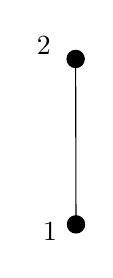
\begin{tikzpicture}[x=0.75pt,y=0.75pt,yscale=-1,xscale=1]
%uncomment if require: \path (0,300); %set diagram left start at 0, and has height of 300

%Shape: Circle [id:dp8298753983931657] 
\draw  [fill={rgb, 255:red, 0; green, 0; blue, 0 }  ,fill opacity=1 ] (91.34,170.7) .. controls (91.34,168.4) and (93.2,166.53) .. (95.5,166.53) .. controls (97.8,166.53) and (99.67,168.4) .. (99.67,170.7) .. controls (99.67,173) and (97.8,174.87) .. (95.5,174.87) .. controls (93.2,174.87) and (91.34,173) .. (91.34,170.7) -- cycle ;
%Shape: Circle [id:dp35059080828673506] 
\draw  [fill={rgb, 255:red, 0; green, 0; blue, 0 }  ,fill opacity=1 ] (91.17,91) .. controls (91.17,88.7) and (93.03,86.83) .. (95.33,86.83) .. controls (97.63,86.83) and (99.5,88.7) .. (99.5,91) .. controls (99.5,93.3) and (97.63,95.17) .. (95.33,95.17) .. controls (93.03,95.17) and (91.17,93.3) .. (91.17,91) -- cycle ;
%Straight Lines [id:da45194945483637716] 
\draw    (95.33,91) -- (95.5,170.7) ;



% Text Node
\draw (83,174.33) node    {$1$};
% Text Node
\draw (80,84.67) node    {$2$};


\end{tikzpicture}
\end{document}
